%%Section4-5

\section{実験装置}
\begin{figure}[h]
  \begin{center}
    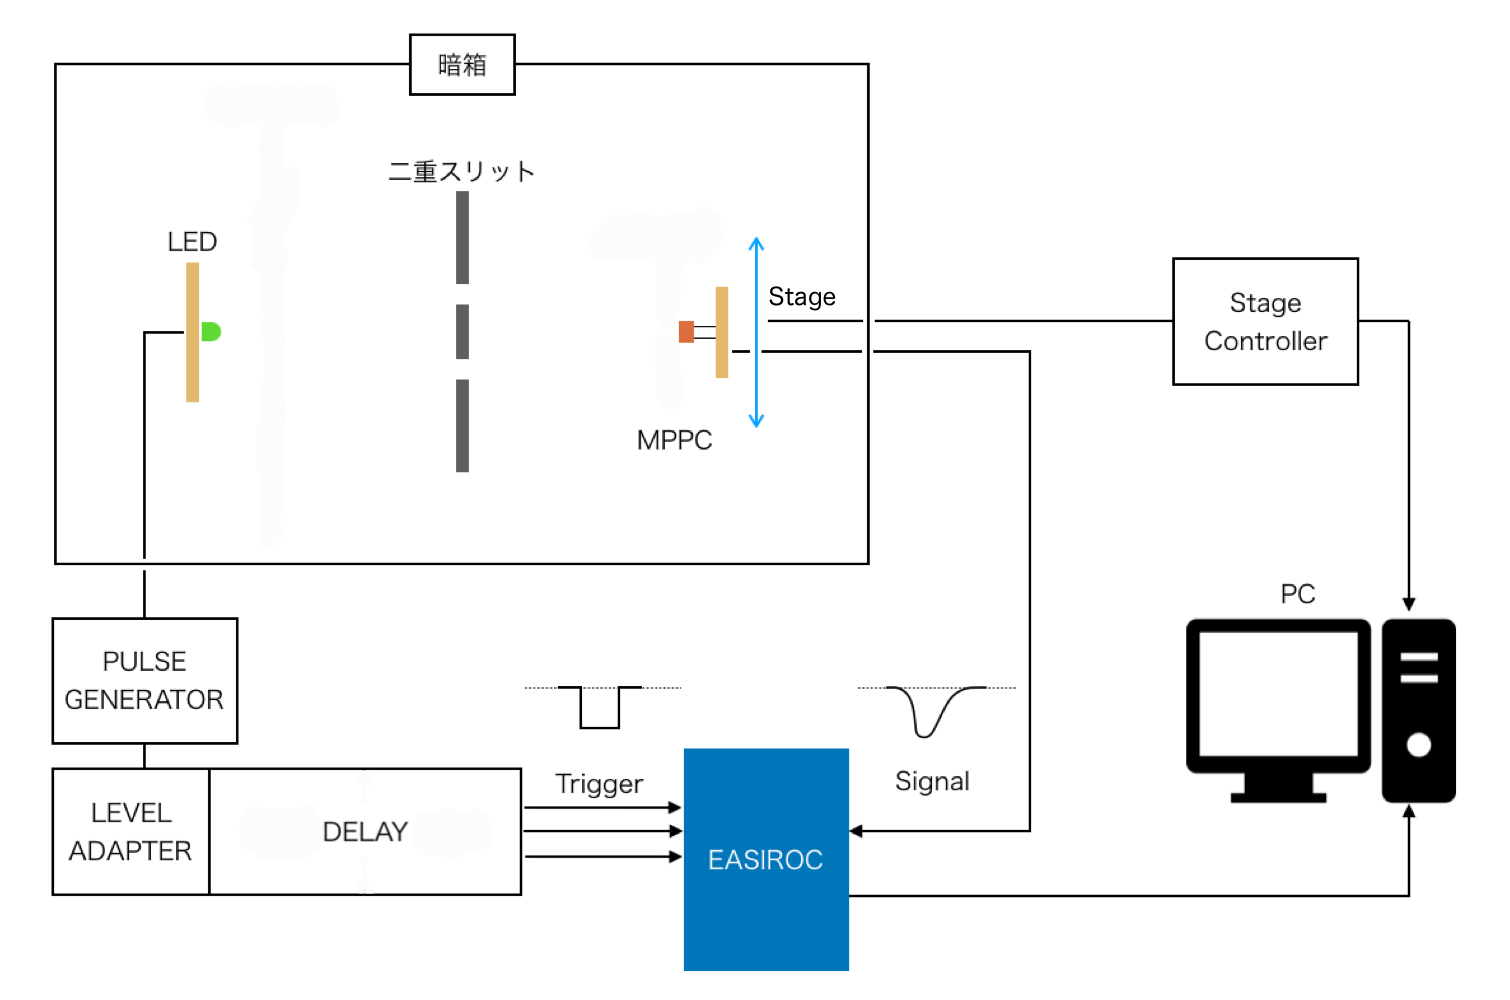
\includegraphics[width=12cm]{../setup_2021.jpeg}
  \end{center}
  \caption{実験の模式図}
\end{figure}

本実験で用いる実験装置.
\begin{itemize}
	\item LED 光源
	\item MPPC 光検出器
	\item PULSE GENERATOR 波高発生器. 非常に高い周期(1kHz)で矩形波を出力.出力と同期してトリガーを出力することも可能.
	\item EASIROC  MPPC読み出しモジュール
	\item スリット  
	\item 可動ステージ 「Stage Controller」で制御.MPPCが設置されている基盤の位置を可動式ステージで細かく変更することが可能.
	 \item 測定用PC EASIROCの制御や, 可動式ステージの制御を行う.データ取得まで行うことができる.
	 \item NIMモジュール
\begin{description}
  		\item[LEVEL ADAOTER] レベルアダプター.TTL 入力信号をNIM 信号に変換し, 出力.
  		\item[DELAY] 遅延回路.信号を遅らせるもの.要は長いケーブル.
\end{description}
\end{itemize}
光学機器を図のように並べ, 光の干渉を起こす.各デバイスの位置や距離によって干渉の見え方が変わるが, これは実際に物を置いていろいろ試してみるとよい.以下では, 光検出器とその読み出しについて説明する.

\subsection{光検出器}
光センサにはたくさんの種類があるが,どれも光を電気信号に変換して取り出すという点は共通している.
今回の実験で用いるのはMPPCと呼ばれる優れた光子カウント能力を持つ小型の光検出器である.

\subsubsection{半導体}
半導体の電気伝導度は金属と絶縁体の中間の値をとり,温度,光,および微量の不純物に対し非常に敏感である.
半導体のエネルギーギャップは1eV程度で, 0 Kではすべての電子は価電子帯にあり伝導帯は空である.室温(かつ通常の圧力)では,エネルギーギャップは室温の熱エネルギー$k_BT$の数十倍であり,かなりの数の電子が価電子帯から伝導帯へ熱的に励起される.
不純物の数が熱的に励起された電子正孔の数より少ない半導体を真性半導体という.GeやSiがあるが,実用的にはSiデバイスが使われている.
真性半導体では伝導帯の電子密度と価電子帯の正孔密度は等しい.
半導体に不純物をドープすると,不純物準位が生じる.
Si原子が価電子5の原子(例えばAs)に置換されると$n$型半導体,価電子3の原子(例えばB)に置換されると$p$型半導体になる.ここでAsをドナー,Bをアクセプタという.
$n$型半導体の多数キャリアは電子(少数キャリアは正孔),$p$型半導体の多数キャリアは正孔(少数キャリアは電子)である.

\subsubsection{pn接合}
$p$型半導体と$n$型半導体を接合すると,接合部における大きなキャリアの密度勾配によって,キャリアの拡散が起こる.
$p$側から$n$側に向かって正孔が,$n$側から$p$側に向けて電子が拡散する.
正孔が$p$側から移動すると,アクセプタ原子のマイナスイオンが接合近傍に残る.
同様に,電子が$n$側から移動すると,ドナー原子のプラスイオンが接合近傍に残る.
その結果,接合部分で自由キャリアが欠乏し,空間電荷ができ,$n$側から$p$側の向きの電場が発生する.$p$側,$n$側の中性領域の電位差を内蔵電位という.
この電場によるドリフト電流は,拡散電流と逆である.すなわち,熱平衡状態において,接合面を通過する実効的な電流はゼロである.
キャリアの拡散によりイオン化した領域のキャリアはゼロであり,空乏層(空間電荷領域)と呼ばれる.

pn接合に外部電場をかけた場合を考える.$n$側に正の電圧$V_R$を加えると,逆方向にバイアスされたことになり,接合面を挟んだ静電ポテンシャルは$V_{bi}+V_R$となる.
空乏層幅$W$を外部電場$V$(逆方向のとき負)で記述すると,
\begin{equation}
W=\sqrt{\frac{2\epsilon_s(V_{bi}-V)}{qN_B}}
\end{equation}
で,空乏層幅$W$は,接合両側の電位差の平方根に比例する.したがって,逆方向バイアスによって,空乏層幅は大きくなる.

\begin{figure}[h]
  \begin{center}
    \includegraphics[width=12cm]{../pnjunction_IV.png}
  \end{center}
  \caption{典型的なシリコンpn接合の電流電圧特性}\label{fig.pnIV}
\end{figure}

pn接合の理想電流電圧特性を図\ref{fig.pnIV}に示す.逆方向バイアスでは,ある臨界電圧(降伏電圧)に達すると急激に電流が増大する.これを接合の降伏という.
降伏現象の機構は,トンネル効果(ツェナー降伏)となだれ増幅(アバランシェ降伏)がある.
ここではなだれ増幅のみ説明する.

\subsubsection{なだれ(アバランシェ)増幅}

電界強度が十分に強ければ,空乏層内で熱的に励起された電子は,電場(内部+外部)で加速され,格子原子と衝突してその結合手を切り,電子正孔対を作る.
新しく発生した電子と正孔は,それぞれ電場からエネルギーを得て,再び別の電子正孔対を作る.これらの過程がくりかえし起こることをなだれ増幅と呼ぶ.

なだれ増幅を利用してシグナルを増幅させる仕組みのフォトダイオード(光検出器)をAPD(Avalamche Photo Diode)という.
PADの動作モードはノーマルモードとガイガーモードがある.

ノーマルモードは,降伏電圧以下で動作し,ゲイン(増幅率)は100以下,APDに入射した光子数に比例する電荷量を出力する.
ガイガーモードは,降伏電圧以上で動作し,ゲインは$10^6$程度,APDに入射した光子数に無関係の,電圧値に依存した電荷量が出力される.

\subsubsection{MPPC}
MPPC(Micro Pixel Photon Counter)はAPDが多数配列された光検出器である.
ガイガーモードAPDが多数配列することにより, 我々は光子が入射したAPDのチャンネル数だけを数えることで, (pile upはあるものの)光子数をデジタルに数えることができる.
MPPCは,低電圧で動作し,高い増倍率,高い検出効率,高速応答,優れた時間分解能,広い感度波長範囲といった特徴がある.

MPPCは,ガイガーモードAPDとクエンチング抵抗を組み合わせたものを1ピクセルとして,多数のピクセルを2次元に電気的接続をした構造をもっている.
\begin{figure}[h]
  \begin{tabular}{ccc}
    \begin{minipage}[t]{0.33\hsize}
      \begin{center}
        \includegraphics[width=4cm]{../mppc.jpg}
      \end{center}
      \caption{MPPC}
    \end{minipage}
    \begin{minipage}[t]{0.33\hsize}
      \begin{center}
        \includegraphics[width=4cm]{../APDstructure.PNG}
      \end{center}
      \caption{APD}
    \end{minipage}
    \begin{minipage}[t]{0.33\hsize}
      \begin{center}
        \includegraphics[width=4cm]{../QuenchingArray.PNG}
      \end{center}
      \caption{MPPCはAPDを並列に並べたもの}
    \end{minipage}
  \end{tabular}
\end{figure}

MPPCのピクセルは,それぞれが光子の検出時に同じパルスを出力する.
複数のピクセルに光子が入射した場合,それぞれの出力が重ね合わされるため,光子数に応じて出力パルスの高さが変わる.(\ref{fig.MPPCpulse})
ひとつのピクセルに同時に入射した光子が1フォトンでも2フォトンでも,そのピクセルから出力されるパルスの高さは同じである.(1フォトン入った時点でなだれ増幅が飽和状態になりそれ以上増えない)
\begin{figure}[H]
	\begin{tabular}{cc}
		\begin{minipage}[t]{0.5\hsize}
  			\begin{center}
    			\includegraphics[width=6cm]{../MPPCpulse.png}
    			\caption{MPPCの出力パルス波形}\label{fig.MPPCpulse}	
  			\end{center}
		\end{minipage}
		\begin{minipage}[t]{0.5\hsize}
  			\begin{center}
    			\includegraphics[width=6cm]{../MPPCcharge.png}
    			\caption{MPPCの出力電荷量のヒストグラム}\label{fig.MPPCcharge}	
  			\end{center}
		\end{minipage}
	\end{tabular}
\end{figure}

MPPCの出力パルスの高さは電荷量に比例する.図\ref{fig.MPPCcharge}はチャージアンプを用いたMPPCからの出力電荷量の分布である.
これにより,出力の高さと検出光子数を対応させることが可能になる.

浜松ホトニクスのHPに、MPPCの挙動が説明されている.\cite{hamamatsu}

\subsection{EASIROC}
EASIROCモジュールは, 書き換え不可能な集積回路(ASIC)であるEASIROCチップと, EASIROCチップ制御用の書き換え可能な集積回路(FPGA)であるArtix7が搭載された, MPPCの(多チャンネル)読み出しモジュールである.今回は1チャンネルしか使わないし, FPGAのfirmwareの書き換えも(おそらく)ないので, ここでは, EASIROCチップの回路の概要と, アナログな出力波形について見ることにする.\\
EASIROCチップは, Pre-Amp,Shaper,Discriminator,Capacitorからなる.Pre-Amp,Slow Shaperを通った信号電圧をCapacitorに保存し, Trigger信号が入力されたときに電圧をholdし, ADC(Analog Digital Converter)でデジタル情報に変換する.
\begin{figure}[H]
  \begin{center}
    \includegraphics[width=12cm]{../EASIROCCircuitDiagram.PNG}
  \end{center}
  \caption{EASIROC回路概略}
\end{figure}

\begin{figure}[H]
  \begin{tabular}{cccc}
    \begin{minipage}[t]{0.25\hsize}
      \begin{center}
        \includegraphics[width=4cm]{../preamp.BMP}
      \end{center}
      \caption{Pre-Amp}
    \end{minipage}
    \begin{minipage}[t]{0.25\hsize}
      \begin{center}
        \includegraphics[width=4cm]{../fastshaper.BMP}
      \end{center}
      \caption{Fast Shaper}
    \end{minipage}
    \begin{minipage}[t]{0.25\hsize}
      \begin{center}
        \includegraphics[width=4cm]{../slowshaper.BMP}
      \end{center}
      \caption{Slow Shaper}
    \end{minipage}
    \begin{minipage}[t]{0.25\hsize}
      \begin{center}
        \includegraphics[width=4cm]{../slowshaperhold.BMP}
      \end{center}
      \caption{holdしたSlow Shaper}
    \end{minipage}
  \end{tabular}
\end{figure}


各デバイスを通った信号の出力波形は, EASIROCモジュールのProbe出力を観察するとわかる.Fast ShaperはSelf Trigger用なので, 今回は(おそらく)使わない.Trigger信号に合わせてShaperの波高の一番高いところが読み出されているのがわかる.Trigger信号とShaperの立ち上がりがきちんと合うかどうかはケーブルの長さやDelayモジュールによって操作できる.

\clearpage
\section{測定方法}

\subsection{可動式ステージの使用方法}

可動式ステージは, stage.pyを用いて制御する.使用するためのコマンドは, 以下の通りである.
\begin{figure}[H]
  \begin{lstlisting}[caption=stage.pyのコマンド]
$ ./stage.py [コマンド]  
  \end{lstlisting}
\end{figure}


\begin{table}[H]
  \begin{center}
    \caption{stage.py コマンド一覧}
    \begin{tabular}{|l|l|l|} \hline
      入力コマンド & 使い方       & 動作                                      \\ \hline \hline
      -o           & -o           & left or right 側の原点に戻る              \\ \hline
      -r           & -r           & データリセット, 現在地を原点とする        \\ \hline
      -mr          & -mr [整数値] & 今いるところから[整数値]パルス分+側へ移動 \\ \hline
      -ml          & -ml [整数値] & 今いるところから[整数値]パルス分-側へ移動 \\ \hline
      -pr          & -pr [整数値] & 絶対的な座標位置+[整数値]パルスへ移動     \\ \hline
      -pl          & -pl [整数値] & 絶対的な座標位置-[整数値]パルスへ移動     \\ \hline
      -s           & -s           & 動作停止                                  \\ \hline
      -q           & -q           & ステージの情報を表示                      \\ \hline
      -h           & -h           & コマンドの使い方表示                      \\ \hline
    \end{tabular}
  \end{center}
\end{table}

\begin{itembox}[l]{注意事項}
  \begin{itemize}
    \item 動く距離とパルスの関係は2μm/パルス.
    \item 一度の操作で送ることのできるコマンドは1つ.
    \item 複数送った場合, コマンド一覧の上から順に優先順位がついており, 優先順位が最も高いものの動作を行う.
  \end{itemize}
  例えば, {\tt \$ ./stage.py -ml 1000 -mr 20000 -s -o +} とコマンドを送っても, {\tt -o} のみが認識される.
\end{itembox}

可動式ステージの仕様について詳しくは\cite{movingstage}


\subsection{EASOROCの使用方法}

\subsubsection{EASIROCモジュールへのアクセス}
\begin{lstlisting}
$ ./Controller.rb 192.168.10.102
\end{lstlisting}
でEASIROCモジュールとのシェル上での対話が可能になる.
利用できる主なコマンドは表\ref{table:easiroc_controller_commands}の通りである.
詳しい情報は\href{https://ppwww.phys.sci.kobe-u.ac.jp/~hamada/easiroc_manual.html}{ここのリンク}を参照.

\subsubsection{印加電圧の設定}

たとえば, コントローラを起動したシェルで
\begin{lstlisting}
$ setHV 10
\end{lstlisting}
を実行することでMPPCにバイアス電圧10Vが印加される.
setHVコマンドの実行後は
\begin{lstlisting}
$ statusHV
\end{lstlisting}
を用いてMPPCにかかっている実際のバイアス電圧と電流を確認すること.
光漏れなどの原因によりMPPCに異常な電流が流れていないかを確認することが主な目的である.

\begin{itembox}[l]{注意事項}
  \begin{itemize}
    \item 電流は正常な値で数$\mathrm{\mu A}$程度である.10 倍以上の電流が流れるようであればすぐにsetHV 0 を実行し, 大電流が流れた原因を考えること
  \end{itemize}
\end{itembox}

\begin{table}[htbp]
  \begin{center}
    \caption{easiroc コマンド一覧}
    \label{table:easiroc_controller_commands}
    \begin{tabular}{|l|l|} \hline
      入力コマンド & 動作                                                     \\ \hline \hline
      setHV [bias voltage] & HVを[bias voltage]の値にセットする\\ \hline
      statusHV & HVの電圧と電流を表示する\\ \hline
      read [EventNum] [Filename] & データ取得を行う \\ \hline
      exit, quit & プログラムの終了\\ \hline
    \end{tabular}
  \end{center}
\end{table}

\subsubsection{EASIROC測定手順}
\begin{enumerate}
  \item Controller.rbを用いてEasirocに接続
  \item HG outからの出力をみながら電圧を設定
  \item readコマンドを打って測定開始
\end{enumerate}
測定データはController.rbがあるディレクトリ配下のdataディレクトリ以下に保存される.
測定データの確認方法は以下の通りである.
\begin{lstlisting}
$ cd data
$ root filename.root
root> TBrowser t
\end{lstlisting}
または
\begin{lstlisting}
$ cd data
$ root filename.root
root> ADC_HIGH_12->Draw()
\end{lstlisting}
